\documentclass[12pt,letterpaper]{article}
\usepackage[utf8]{inputenc}
\usepackage[spanish, es-tabla]{babel}
\usepackage[version=3]{mhchem}
\usepackage[journal=jacs]{chemstyle}
\usepackage{amsmath}
\usepackage{amsfonts}
\usepackage{amssymb}
\usepackage{makeidx}
\usepackage{esvect}
\usepackage{xcolor}
\usepackage[stable]{footmisc}
\usepackage[section]{placeins}
%Paquetes necesarios para tablas
\usepackage{longtable}
\usepackage{array}
\usepackage{xtab}
\usepackage{multirow}
\usepackage{colortab}
%Paquete para el manejo de las unidades
\usepackage{siunitx}
\sisetup{mode=text, output-decimal-marker = {,}, per-mode = symbol, qualifier-mode = phrase, qualifier-phrase = { de }, list-units = brackets, range-units = brackets, range-phrase = --}
\DeclareSIUnit[number-unit-product = \;] \atmosphere{atm}
\DeclareSIUnit[number-unit-product = \;] \pound{lb}
\DeclareSIUnit[number-unit-product = \;] \inch{"}
\DeclareSIUnit[number-unit-product = \;] \foot{ft}
\DeclareSIUnit[number-unit-product = \;] \yard{yd}
\DeclareSIUnit[number-unit-product = \;] \mile{mi}
\DeclareSIUnit[number-unit-product = \;] \pint{pt}
\DeclareSIUnit[number-unit-product = \;] \quart{qt}
\DeclareSIUnit[number-unit-product = \;] \flounce{fl-oz}
\DeclareSIUnit[number-unit-product = \;] \ounce{oz}
\DeclareSIUnit[number-unit-product = \;] \degreeFahrenheit{\SIUnitSymbolDegree F}
\DeclareSIUnit[number-unit-product = \;] \degreeRankine{\SIUnitSymbolDegree R}
\DeclareSIUnit[number-unit-product = \;] \usgallon{galón}
\DeclareSIUnit[number-unit-product = \;] \uma{uma}
\DeclareSIUnit[number-unit-product = \;] \ppm{ppm}
\DeclareSIUnit[number-unit-product = \;] \eqg{eq-g}
\DeclareSIUnit[number-unit-product = \;] \normal{\eqg\per\liter\of{solución}}
\DeclareSIUnit[number-unit-product = \;] \molal{\mole\per\kilo\gram\of{solvente}}
\usepackage{cancel}
%Paquetes necesarios para imágenes, pies de página, etc.
\usepackage{graphicx}
\usepackage{lmodern}
\usepackage{fancyhdr}
\usepackage[left=1cm,right=1cm,top=2cm,bottom=3cm]{geometry}

%Instrucción para evitar la indentación
%\setlength\parindent{0pt}
%Paquete para incluir la bibliografía
\usepackage[backend=bibtex,style=chem-acs,biblabel=dot]{biblatex}
\addbibresource{references.bib}

%Formato del título de las secciones

\usepackage{titlesec}
\usepackage{enumitem}
\titleformat*{\section}{\bfseries\large}
\titleformat*{\subsection}{\bfseries\normalsize}

%Creación del ambiente anexos
\usepackage{float}
\floatstyle{plaintop}
\newfloat{anexo}{thp}{anx}
\floatname{anexo}{Anexo}
\restylefloat{anexo}
\restylefloat{figure}

%Modificación del formato de los captions
\usepackage[margin=10pt,labelfont=bf]{caption}

%Paquete para incluir comentarios
\usepackage{todonotes}

%Paquete para incluir hipervínculos
\usepackage[colorlinks=true, 
            linkcolor = blue,
            urlcolor  = blue,
            citecolor = black,
            anchorcolor = blue]{hyperref}

%%%%%%%%%%%%%%%%%%%%%%
%Inicio del documento%
%%%%%%%%%%%%%%%%%%%%%%

\begin{document}
\renewcommand{\labelitemi}{$\checkmark$}

\renewcommand{\CancelColor}{\color{red}}

\newcolumntype{L}[1]{>{\raggedright\let\newline\\\arraybackslash}m{#1}}

\newcolumntype{C}[1]{>{\centering\let\newline\\\arraybackslash}m{#1}}

\newcolumntype{R}[1]{>{\raggedleft\let\newline\\\arraybackslash}m{#1}}

\begin{center}
	\textbf{\LARGE{Práctico 1 - Redes Neuronales 2020}}\\
	\vspace{7mm}
		\textbf{\large{FAMAF - UNC}}\\
	\vspace{4mm}
	\textbf{\large{Alumno: Pablo N. Rosa}}\\
	\textbf{\large{Profesor: Francisco A. Tamarit}}\\
\end{center}

\vspace{4mm}

\section{Introducción}

Las ecuaciones de \textbf{Lotka-Volterra}, también conocidas como \textbf{ecuaciones predador-presa} o \textbf{presa-predador}, son un par de ecuaciones diferenciales de primer orden no lineales que se usan para describir dinámicas de sistemas biológicos en el que dos especies interactúan, una como \textit{presa} y otra como \textit{depredador}. Las ecuaciones fueron propuestas de forma independiente por \textit{Alfred J. Lotka} en 1925 y \textit{Vito Volterra} en 1926. 

Tales ecuaciones se definen como:

$$\dot{C}(t) = \alpha C(t) - \beta C(t)Z(t)$$
$$\dot{Z}(t) = -\gamma Z(t) + \delta C(t)Z(t)$$

La función $C(t)$ modela el
número de conejos (presa) en un ecosistema dado, y $Z(t)$ la cantidad de zorros (depredador) en el mismo ecosistema. 

La primera ecuación puede interpretarse como el cambio del número de presas dado por su propio crecimiento menos la tasa de encuentros con predadores. Mientras que la segunda ecuación, se puede interpretar como el crecimiento de los depredadores por la caza de presas menos la muerte natural de estos.

Para estudiar el comportamiento de este sistema, se aplicarán los métodos numéricos y cualitativos vistos en clase.

\section{Análisis y resultados}

\subsection{Análisis cualitativo}

Para el caso que analizaremos los parámetros toman los siguientes valores:
$$ \alpha= 0.1 \quad \beta = 0.02, \quad \gamma = 0.3 \quad y \quad  \delta = 0.01$$

Además para seguir la convención dada y simplicar la notación, se escribirá el sistema anterior prescidiendo del parámetro $t$, es decir, $C(t) = C$ y $Z(t) = Z$ por lo que el sistema resultante es:

$$\dot{C} =  0.1 C - 0.02 CZ $$
$$\dot{Z} = -0.3 Z + 0.01 CZ $$

Notemos que este sistema sólo tiene sentido físico para valores positivos de $C$ y $Z$, ya que no puede haber un número negativos de animales. 

El primer paso consiste en linealizar el sistema, para lo cual se computa el Jacobiano.

$$A = 
\begin{bmatrix}
\dfrac{\partial \dot{C}}{\partial C} & \dfrac{\partial \dot{C}}{\partial Z} \\
 & \\
\dfrac{\partial \dot{Z}}{\partial C} & \dfrac{\partial \dot{Z}}{\partial Z} 
\end{bmatrix} 
= 
\begin{bmatrix}
0.1 - 0.02 Z & -0.02 C \\
0.01 Z & -0.3 + 0.01 C  
\end{bmatrix}
$$

El próximo paso consiste en buscar los \textbf{puntos fijos},  es decir, los $(x^*, y^*)$ que simultáneamente satisfacen que:

$$\dot{C} = 0 \quad y \quad \dot{Z} = 0 $$

Notemos que:

$$0.1 C - 0.02 CZ = C(0.1 - 0.02 Z) = 0 \quad (1)$$
$$−0.3 Z + 0.01 CZ = Z(-0.3 - 0.01 C) = 0 \quad (2)$$

Por lo tanto un punto fijo es $P_1 = (0, 0)$. 

El otro punto fijo $P_2$, se obtiene por $(1)$ y $(2)$: 

$$C(0.1 - 0.02 Z) = 0 \iff (0.1 - 0.02 Z) = 0 \iff 0.1 = 0.02 Z \iff Z = \dfrac{0.1}{0.02} = 5$$ 
$$Z(-0.3 + 0.01 C) = 0 \iff (-0.3 + 0.01 C) = 0 \iff 0.3 = 0.01 C \iff C = \dfrac{0.3}{0.01} = 30 $$ 

Luego $P_2 = (30, 5)$. 

En el tercer paso se computa el el jacobiano en cada punto fijo y viendo sus autovalores y autovectores, analizamos su naturaleza y estabilidad:

\begin{itemize} 
\item La matriz evaluada en el punto $P_1 = (0, 0)$ es 
$$A = \begin{bmatrix}
0.1 & 0 \\
0 & -0.3   
\end{bmatrix}$$

Sus autovalores son: $\lambda_1 = 0.1$ y $\lambda_2 = -0.3$ y los autovectores correspondentes son: $\vv{v_1} = \begin{bmatrix}1 \\ 0\end{bmatrix}$ y $\vv{v_2} = \begin{bmatrix}0 \\ 1\end{bmatrix}$. Estos resultados muestran que este punto de equilibrio es un \textbf{punto de silla} (\textit{saddle node}) con soluciones que crecen exponencialmente a lo largo del eje $C$ y decrecen a lo largo del eje $Z$.
\end{itemize}

\begin{itemize}
\item La matriz evaluada en el punto $P_2 = (30, 5)$ es 
$$A = \begin{bmatrix}
0 & -0.6 \\
0.05 & 0   
\end{bmatrix}$$

Para esta matriz calculamos que sus autovalores son \textit{imaginarios puros} (sin parte real): $\lambda_1, \lambda_2 = \pm \sqrt{0.03} i = \pm \sqrt{\alpha \gamma} i $. Por esto todas las soluciones son períodicas con período $T = \dfrac{2\pi}{\alpha \gamma} = \dfrac{2\pi}{0.03}$. Las oscilaciones tienen un amplitud fija y el punto fijo es un \textbf{centro}.

\end{itemize}

Finalmente para esbozar el diagrama de fase, es útil trazar las líneas nulas (\textit{nullclines}), definidas como
curvas donde $\dot{N} = 0$ o $\dot{Z} = 0$. En los los los puntos en donde $\dot{N} = 0$ sólo tendremos vectores con componentes verticales y en los puntos tales que $\dot{Z} = 0$ tendremos vectores con componentes horizontales. Mirando el signo de las otras derivadas sabremos el sentido de los vectores (abajo/arriba o derecha/izquierda).   

De las ecuaciones $(1)$ y $(2)$, tenemos que las las $C-nullclines$ son $C = 0$ y $Z = 5$ mientras que las $Z-nullclines$ son $Z = 0$ y $C = 30$. El signo de las derivadas para cada nullclines es:

\begin{itemize}
\item Para las $\textbf{C-nullclines}$:
\begin{itemize}

\item Si $C = 0$ entonces $\dot{Z} = -0.3Z < 0$.
\item Si $Z = 5$ entonces $\dot{Z} = -1.5  + 0.05C > 0 \iff C > 30$ Y $\dot{Z} = -1.5  + 0.05C < 0 \iff C < 30$.
\end{itemize}
\item Para las $\textbf{Z-nullclines}$:
\begin{itemize}
\item Si $Z = 0$ entonces $\dot{C} = 0.1C > 0$.
\item Si $C = 30$ entonces $\dot{C} = 3 - 0.6Z > 0 \iff Z < 5$ Y $\dot{C} = 3  - 0.6Z < 0 \iff Z > 5$.
\end{itemize}

\end{itemize}

Esto divide al grafico en cuatro cuadrantes alrededor del centro $P_2$ y graficando vectores en cada uno de ellos, queda definido el sentido de rotación como antihorario. Esto se muestra en la parte izquierda de la Figura 1.

\begin{figure}[h!]
\begin{floatrow}
\centering
\caption{Gráficos del análisis cualitativo}
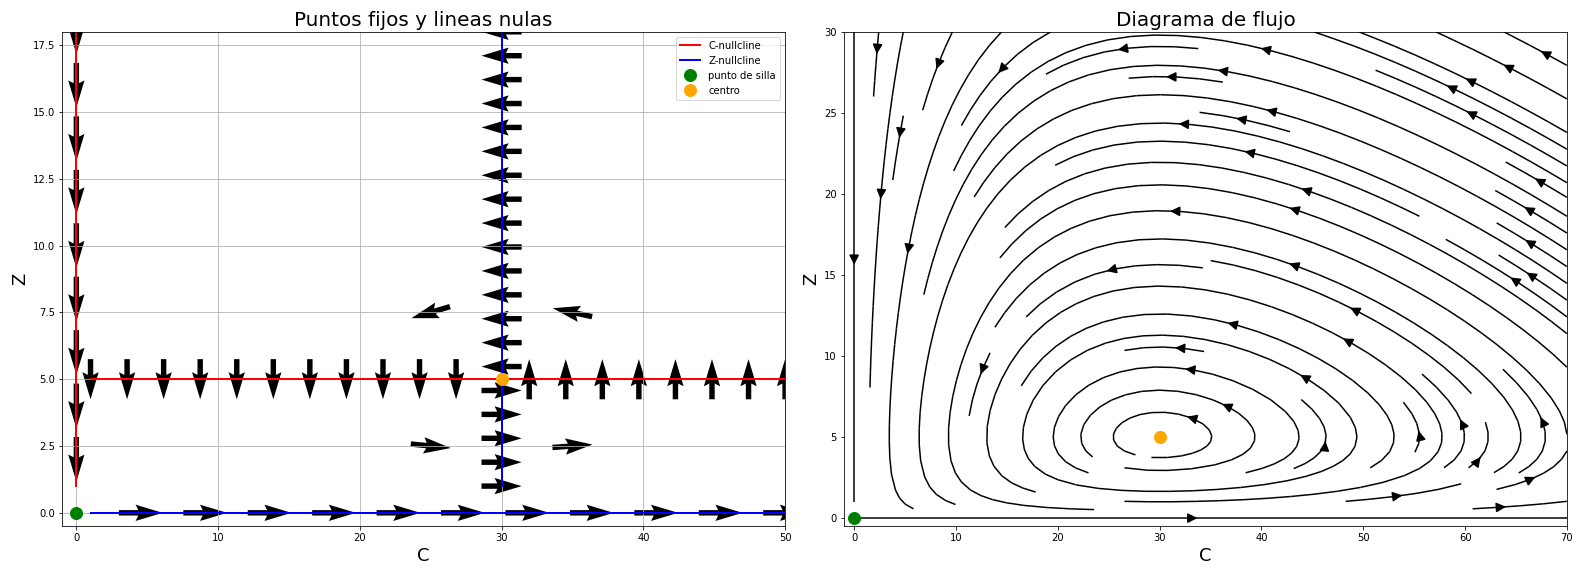
\includegraphics[width=20cm]{./images/rabbits_and_foxes_2.png}
\label{fig:esquema}
\end{floatrow}
\end{figure}

En la derecha de la Figura 1, se observa el diagrama de flujo resultante. El punto silla (origen) es un punto de equilibrio en donde no hay presas ni depredadores y nunca los habrá. Además si en el instante inicial, una de las variables es nula, si la no nula es presa, entonces aumenta porque no hay quien la deprede; mientras que si es depredador, dismimuye hasta desaparecer por inanición. En el punto que es centro, se tiene un caso en donde las conejos son devorados por los zorros, y ambas poblaciones se mantienen estables en número. Esta última situación es muy poco probablemente, y lo que predomina es la variación cíclica del número de especies: si hay un gran número de conejos y pocos zorros, entonces los últimos podrán alimentarse bien y se reproducirán; en algún punto habrá mas zorros que conejos, por lo que el alimento no será suficiente, haciendo que su número disminuya, por muerte y menos reproducción. Con esto, los conejos menos amenazados podrán aumentar de nuevo, y se habrá vuelto a la condición inicial. 

\subsection{Análisis numérico}

En esta sección, se encontrará una solución numérica aproximada al problema usando los parámetros del punto anterior, y entre los tiempos  $t=0$  y  $t=200$ con un paso de integración  $h=0.05$ y  con condiciones iniciales: $C(0)=40$ y $Z(0)=9$.
 
Esto es lo que se conoce como \textit{problema del valor inicial} y puede resolverse usando un métodos iterativos que aproximan las soluciones de estas ecuaciones.

En este caso resolveremos el problema usando el método Runge-Kutta de cuarto orden (RK4).

En la Figura 2, se observa un gráfico paramétrico de $C(t)$ vs $Z(t)$ con las soluciones que brinda el método para estas condiciones iniciales.

\begin{figure}[h!]
\begin{floatrow}
\centering
\caption{Gráficos del análisis numérico}
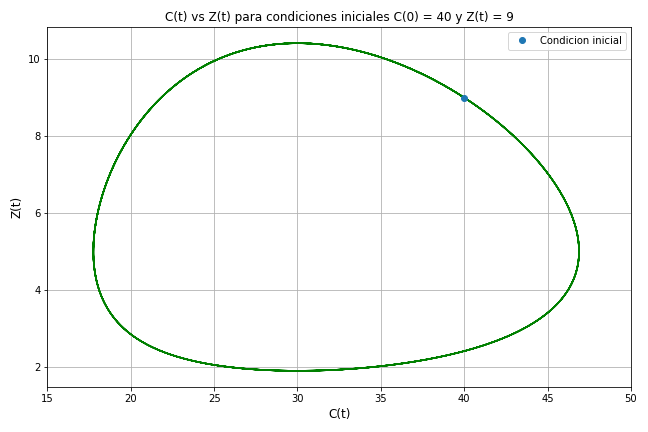
\includegraphics[width=12cm]{./images/rabbits_and_foxes_3.png}
\label{fig:esquema}
\end{floatrow}
\end{figure}

Como el sistema se mueve en sentido antihorario desde las condiciones iniciales, vemos que el sistema pronto alcanzará el máximo número de zorros posibles (un poco más de 10), a la vez que el número de conejos irá descendiendo. A partir de allí, los zorros comenzarán a ser menos y  sus presas también, hasta llegar a un 
mínimo de presas posibles. Desde allí, los conejos aumentarán hasta alcanzar su máximo (algo más de 45), no sin antes haberse alcanzado el mínimo de depredadores. Vemos que los conejos son las base del ecosistema, ya que a su máximo le sigue del máximo de zorros, y a su mínimo le sigue el mínimo de depredadores. Sin embargo con este modelo, estos parámetros y condiciones iniciales, ninguna especie llega a extinguirse, se mantiene el comportamiento periódico que mostró el diagrama de flujo.

\end{document}
